% mainfile: ../../../../master.tex
\subsection{Extraction of total DNA and RNA from marine samples}
% The part of the label after the colon must match the file name. Otherwise,
% conditional compilation based on task labels does NOT work.
\label{task:20180112_cj1}
\tags{lab}
\authors{cj}
%\files{}
%\persons{}


\subsubsection{Introduction}

The starting materials are two different bacterial cultures (kindly given to me by Anouk Lyver):
\begin{itemize}
\item[] \texttt{423 10M1}: few colonies of bacteria isolated from station 423 at 10 m deep on solid media transfered into 2~mL of sterile water.
\item[] \texttt{ALMIX}: a mixture of two liquid cultures that looked very rich in cell number with a final volume of 2~mL.
\item[] \texttt{CTRL}: negative control.
\end{itemize}

I will follow the protocol adapted from \citet{schneider2017extraction} and \citet{chomczynski2006single}.

\subsubsection{Lysis and homogenisation}

\begin{enumerate}
\item 2 mL of cultures are in 2mL-Eppendorf tubes.
\item Centrifuge at 9300 RCF (10000 rpm) at 4\degree C for 10 min (Eppendorf 5415R).
\comment{For both \texttt{423 10M1} and \texttt{ALMIX} I can see a pellet (cf. figure \ref{sfig:20180112_pellet_ALMIX}).} 
\item Remove the supernatent.
\item Add 2 mL of denaturing solution.
\item Vortex.
\item Incubate at room temperature for 10 min.
\item Transfer the lysate into 15mL-Falcon tubes
\end{enumerate}


\begin{figure}[H] % position of the figure 
    \centering
    \caption{Pictures of the samples.}
    \label{fig:20180112_smp}
    \begin{subfigure}[b]{0.49\textwidth}
        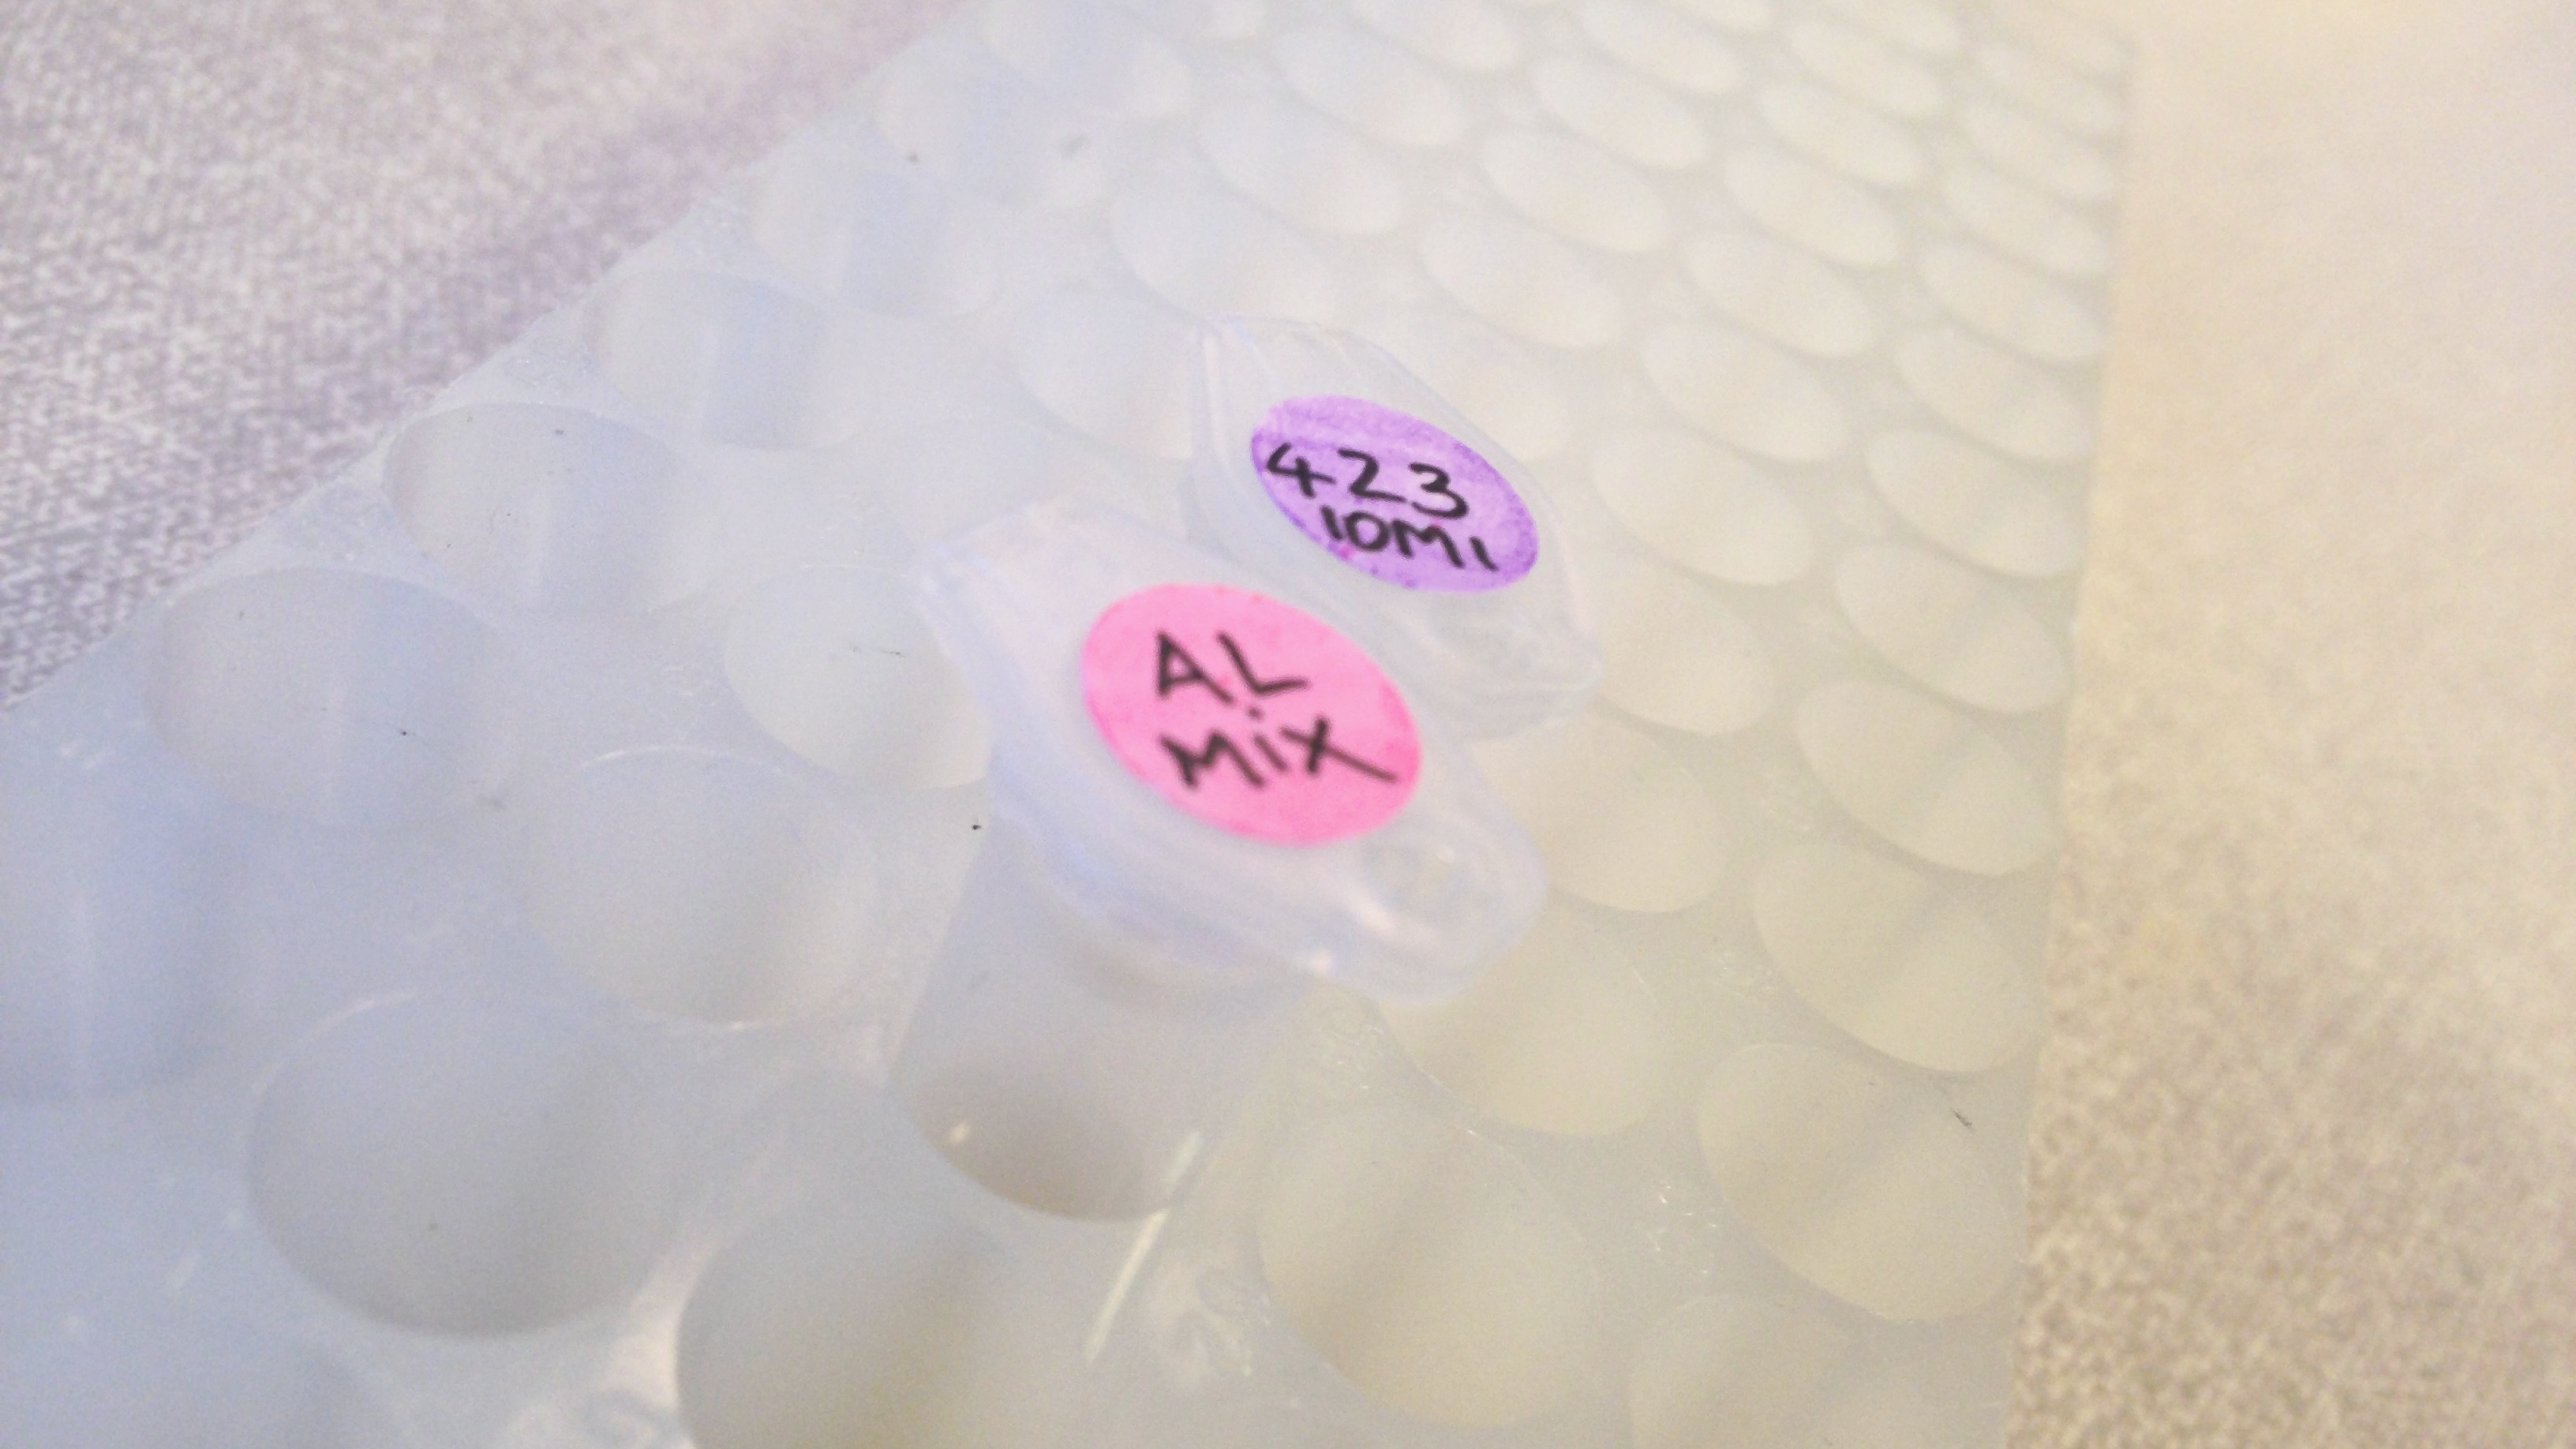
\includegraphics[width=\textwidth]{graphics/pic/20180112_samples.png}
        \caption{Pictures of the labels for the tubes}
        \label{sfig:20180112_samples}
    \end{subfigure}
    ~ 
    \begin{subfigure}[b]{0.49\textwidth}
        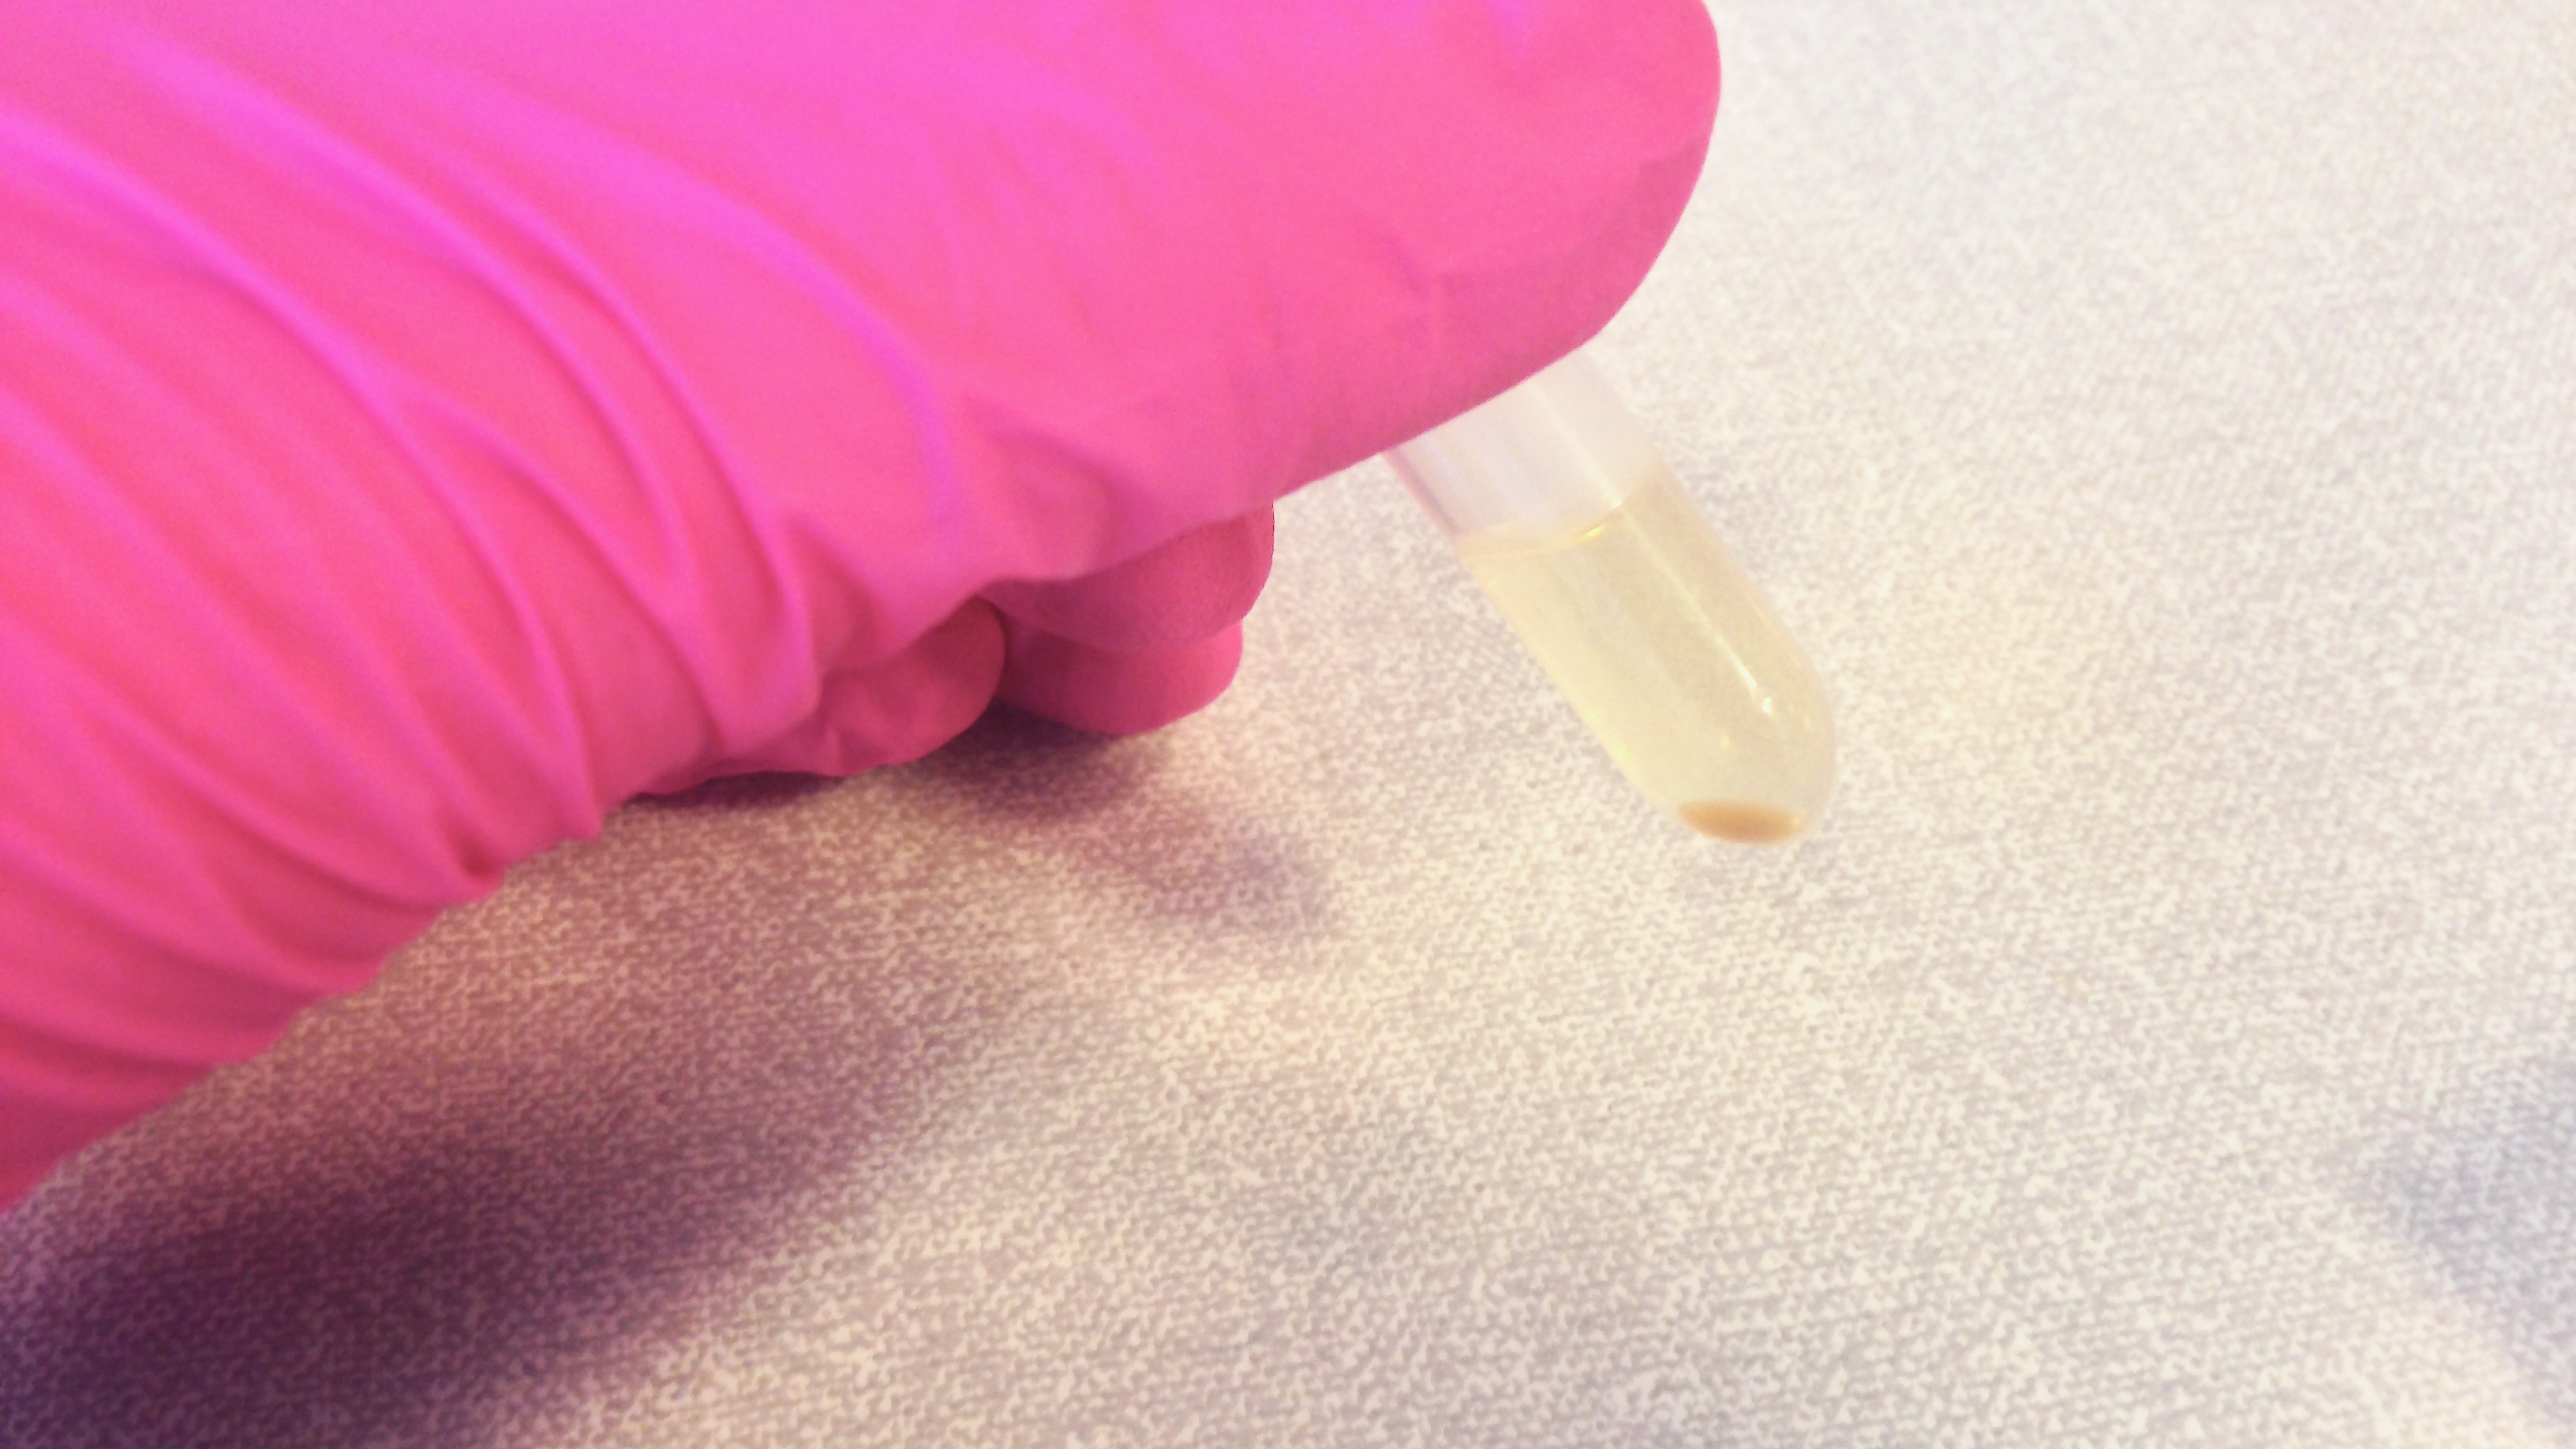
\includegraphics[width=\textwidth]{graphics/pic/20180112_pellet_ALMIX.png}
        \caption{Picture of the pellet observed \texttt{ALMIX}}
        \label{sfig:20180112_pellet_ALMIX}
    \end{subfigure}
\end{figure}

\subsubsection{Simultaneous DNA and RNA extraction}
\begin{enumerate}
\item Add 0.1 volume of 2~M sodium acetate pH 4.
\item Add 1 volume of phenol pH 4.
\sidenote{I always have to bring the bottle of phenol in the teaching lab, which is actually not very safe, but on my way I met Bergrós and Brynja who introduces me a little trolley!}
\item Mix thoroughly by inversion.
\item Add 0.2 volume of chloroform:isoamyl alcohol (24:1).
\item Cool on ice for 15 min.
\item Centrifuge for 20 min at 7200 g at 4\degree C (during the centrifugation, the mixture should separate into a lower phenol phase and interphase and an upper aqueous phase).
\item Transfer carefully the supernatent (aqueous phase) which contains mostly RNA to a clean Falcon tube.
\item Add 2~mL of 2~M sodium acetate buffer pH 4.
\item Mix thoroughly by inversion.
\item Centrifuge for 20 min at 4\degree C.
\item Transfer carefully the upper phase to the already collected aqueous phase.
\item For later DNA isolation, add 1 volume of Tris-base pH 10.5 to the phenolic phase and mix well.
\comment{Here I actually add a lot more Tris-base pH 10.5: I check the pH with pH paper to ensure the pH is back to neutral/alkaline which lead me to have two falcon tubes each containing 14 mL.}
\item Continue with RNA precipitation. 
\end{enumerate}

\subsubsection{RNA isolation}
\begin{enumerate}
\item Add 1 volume of chloroform:isoamyl alcohol (24:1).
\item Incubate at -20\degree C for at least 15 min (but no longer than 1h).
\item Centrifuge again for 20 min at 4\degree C to separate the two phases.
\item Transfer the aqueous upper plase to a frish tube
\item Repeat the chloroform extraction by adding 2~mL of 2~M sodium acetate buffer to the organic phase, mix and centrifuge again, and finally transfer the supernatent to the already collected aqueous phase.
\item Add 1/500 volume of glycogen (20 mg/mL) \sidenote{The glycogen solution was prepared by Stephen back in 2014 and kept at -20\degree C.}
\item Mix vigorously.
\item Add 1 volume of isopropanol to precipitate RNA.
\item Incubate samples at -20\degree C overnight. 
\item Continue with DNA isolation.
\end{enumerate}

\subsubsection{DNA isolation}
\begin{enumerate}
\item Mix tube containing the extracted DNA obtained from previous steps.
\item Centrifuge again for 20 min at 5000 RPM at 4\degree C to separate the two phases.
\item Transfer the upper aqueous phase into fresh tubes (at this point, check pH again with pH paper).
\item Add 2~mL of 1~M Tris-base pH 10.5 to the lower phenolic phase and repeat mixing and centrifugation to separate the two phases.
\item Transfer the upper aqueous phase to the already collected aqueous phase (at this point, check pH again with pH paper).
\item Add 1 volume of chloroform:isoamyl alcohol (24:1) to the aqueous phase.
\item Mix thoroughly by inversion.
\item Centrifuge for 10 min at 4\degree C to separate the two phases/
\item Add 1/500 volume of glycogen (20 mg/mL).
\item Mix thoroughly.
\item Add 2.5 volumes of ice-cold pure ethanol to precipitate the DNA.
\comment{At this stage, for each sample, I have two 15mL-Falcon tubes containing 14~mL.} 
\item Mix thoroughly.
\item Incubate samples at -20\degree C overnight.
\end{enumerate}

\comment{I will leave my samples to incubate overnight because it is getting late and I don't think it will be safe to keep processing the experiment now.}


